\documentclass{article}

\usepackage{graphicx}
\usepackage{tikz}
\usepackage{tikzsymbols}
\usetikzlibrary{calc,patterns,shapes.geometric}
\pagestyle{empty}
\usepackage[margin=0pt]{geometry}
\geometry{papersize={14in,12in}}

\def\centerarc[#1](#2)(#3:#4:#5){\draw[#1] ($(#2)+({#5*cos(#3)},{#5*sin(#3)})$) arc (#3:#4:#5);}

\begin{document}
	\begin{figure}
		\centering
		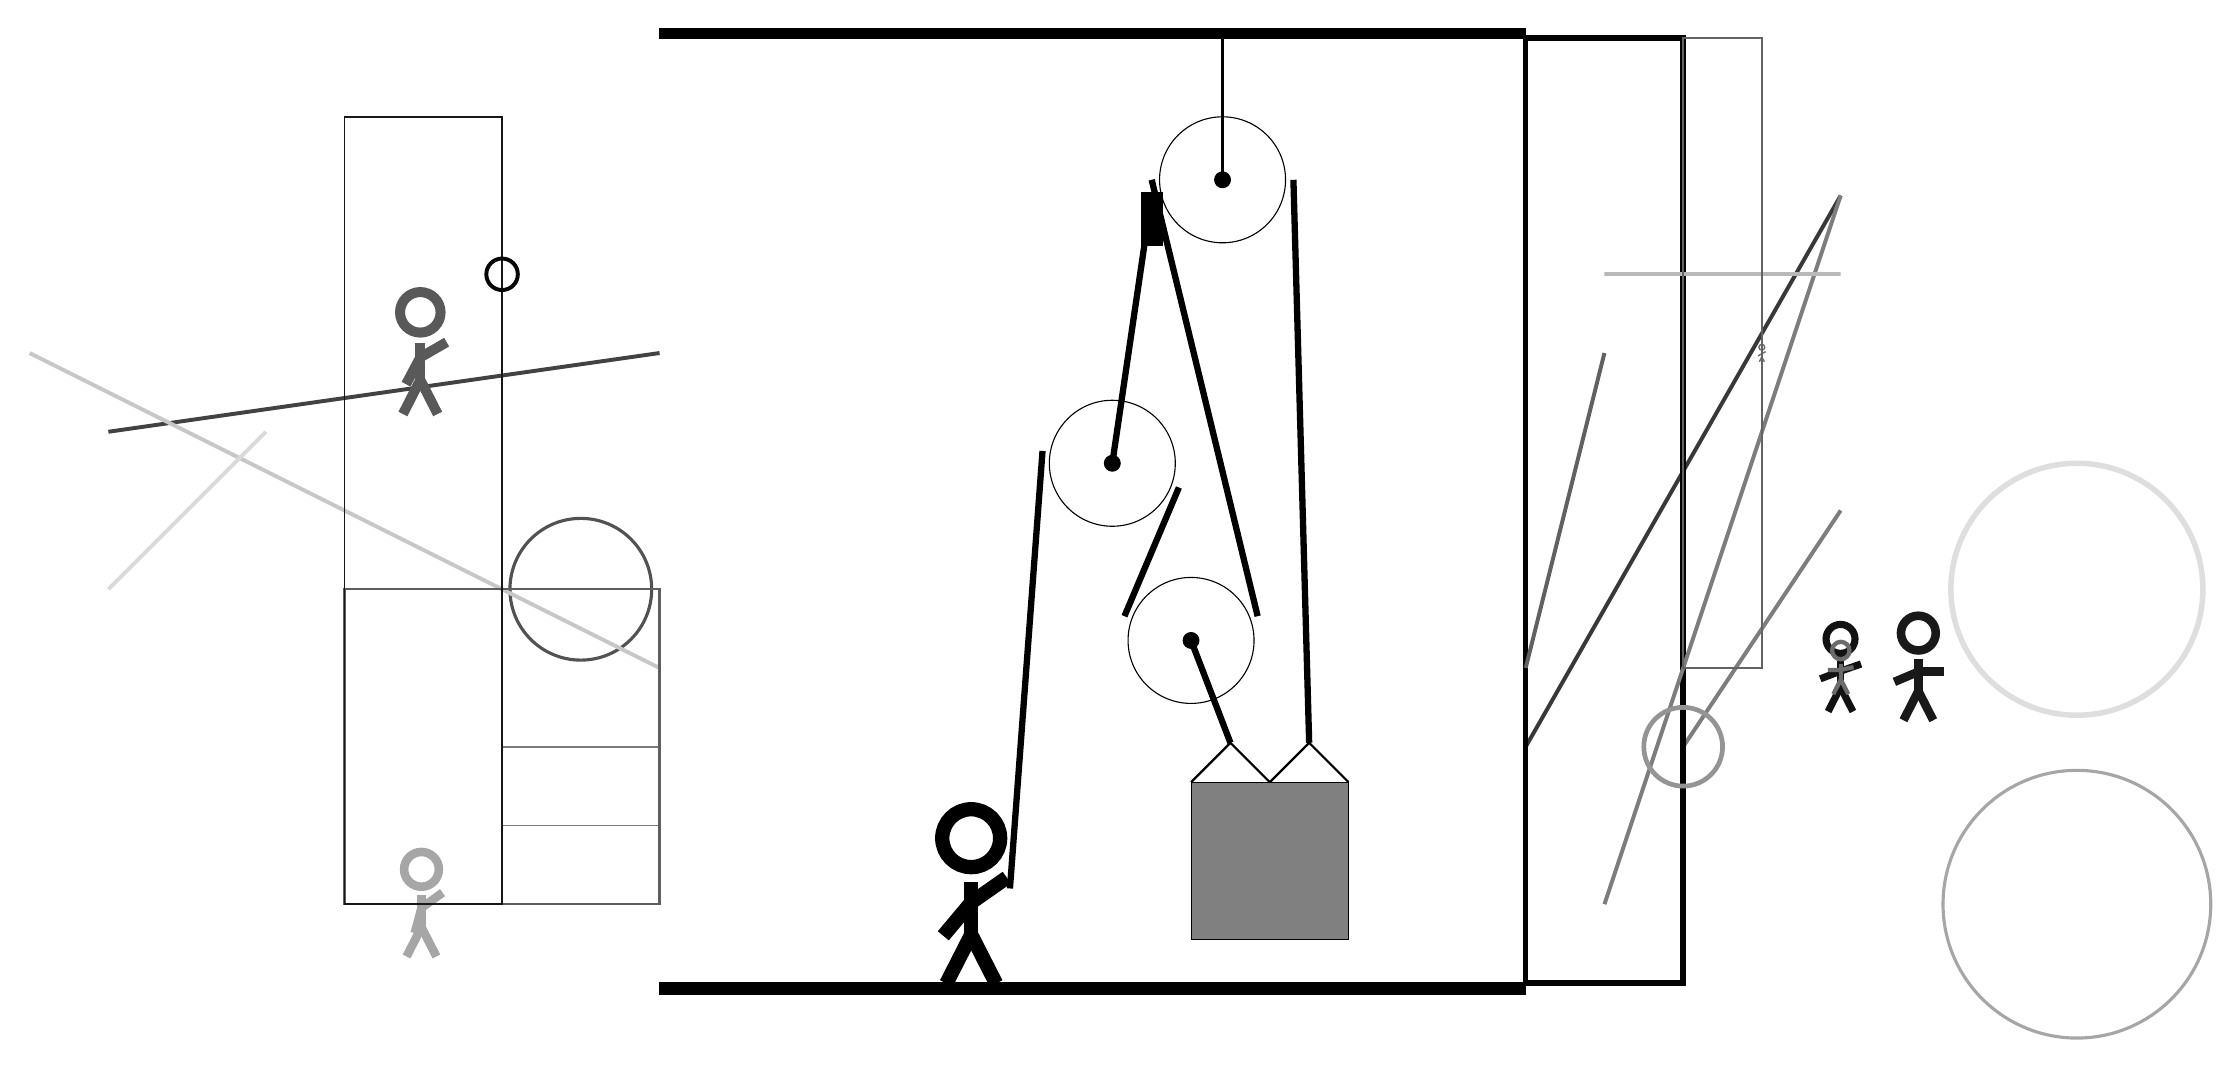
\begin{tikzpicture}
			%%%%% START %%%%%
			
			\draw[fill=black] (-6, 9) rectangle (5, 9.125);
			
			\draw (-0.25, 3.6) circle (0.8);
			\draw[fill=black] (-0.25, 3.6) circle (0.1);
			
			\draw (0.75, 1.35) circle (0.8);
			\draw[fill=black] (0.75, 1.35) circle (0.1);
			
			\draw[line width=0.5mm, color=black!74](-6, 5) -- (-13, 4);
			
			\node[line width=0.2mm, color=black!93] at (9, 1) {\Strichmaxerl[5][21][19]};
			\draw[line width=0.2mm, color=black!52] (-6, -1) rectangle (-8, 0);
			\draw [line width=0.4mm, color=black!68](-7, 2) circle (0.9);
			
			\draw [line width=0.4mm, color=black!35](12, -2) circle (1.7);
			\node[line width=0.6mm, color=black!35] at (-9, -2) {\Strichmaxerl[6][75][36]};
			\draw[line width=0.5mm, color=black!22](-6, 1) -- (-14, 5);
			\node[line width=0.3mm, color=black!90] at (10, 1) {\Strichmaxerl[6][23][0]};
			\draw[line width=0.5mm, color=black!77] (7, 6) rectangle (7, 6);
			
			\node[line width=0.3mm, color=black!65] at (-9, 5) {\Strichmaxerl[7][62][30]};
			
			\draw[line width=0.5mm, color=black!78](9, 7) -- (5, 0);
			\draw[line width=0.5mm, color=black!51](7, 0) -- (9, 3);
			\node[line width=0.2mm, color=black!57] at (8, 5) {\Strichmaxerl[1][32][28]};
			
			\draw[line width=0.7mm, color=black!99] (5, 9) rectangle (7, -3);
			\draw[line width=0.3mm, color=black!63] (-6, -2) rectangle (-10, 2);
			\node[line width=0.2mm, color=black!58] at (9, 1) {\Strichmaxerl[3][1][12]};
			\draw[line width=0.5mm, color=black!51](6, -2) -- (9, 7);
			\draw [line width=0.7mm, color=black!13](12, 2) circle (1.6);
			\draw[line width=0.5mm, color=black!28] (6, 6) rectangle (9, 6);
			\draw[line width=0.5mm, color=black!15](-11, 4) -- (-13, 2);
			\draw[line width=0.5mm, color=black!62](6, 5) -- (5, 1);
			\draw[line width=0.2mm, color=black!91] (-8, -2) rectangle (-10, 8);
			
			\draw [line width=0.5mm, color=black!98](-8, 6) circle (0.2);
			\draw[line width=0.2mm, color=black!61] (7, 1) rectangle (8, 9);
			\draw [line width=0.6mm, color=black!42](7, 0) circle (0.5);
			
			
			\draw (1.15, 7.2) circle (0.8);
			\draw[fill=black] (1.15, 7.2) circle (0.1);
			\draw[very thick] (1.15, 7.2) -- (1.15, 9);
			
			\draw[thick]  (0.75, -0.45) -- (1.25, 0.05) -- (1.75, -0.45) -- (2.25, 0.05) -- (2.75, -0.45);
			\draw[fill=black!50] (0.75, -0.45) rectangle (2.75, -2.45);
			
			\draw[line width=0.8mm] (-0.25, 3.6) -- (0.25, 7.0);
			\draw[line width=0.8mm, fill=black](0.15, 6.4) rectangle (0.35, 7.0);
			\draw[line width=0.8mm] (-1.55, -1.8) -- (-1.1363, 3.7562);
			\centerarc[line width=0.8mm](-0.25, 3.6)(-20:170:0.9);
			\draw[line width=0.8mm] (0.5957, 3.2922) -- (-0.0957, 1.6578);
			\centerarc[line width=0.8mm](0.75, 1.35)(160:380:0.9);
			\draw[line width=0.8mm] (1.5957, 1.6578) -- (0.25, 7.2);
			\draw[line width=0.8mm](0.75, 1.35) -- (1.25, 0.05);
			\centerarc[line width=0.8mm](1.15, 7.2)(0:180:0.9);
			\draw[line width=0.8mm] (2.05, 7.2) -- (2.25, 0.05);
			
			\node at (-2, -1.9) {\Strichmaxerl[10][50][35]};
			
			\draw[fill=black] (-6, -3) rectangle (5, -3.15);
			
			%%%%% END %%%%%
		\end{tikzpicture}
	\end{figure}	
\end{document}